\documentclass[nonacm,sigconf,natbib=false]{acmart}

% Command definition
\AtBeginDocument{
  \providecommand\BibTeX{{Bib\TeX}}
}

% Remove paragraph indentation, add space between paragraphs
\setlength{\parindent}{0pt}
\setlength{\parskip}{0.5em}

% Metadata Information => No Copy right for us
\setcopyright{none}

\usepackage{listings}
\usepackage{xcolor}
\usepackage{grffile}
\usepackage{float}
\usepackage{array}


\lstdefinestyle{tree}{
    basicstyle=\ttfamily\small,
    columns=fullflexible,
    keepspaces=true,
    frame=single,
    breaklines=true,
    showstringspaces=false
}


\begin{document}

\title{Document Image Binarization Pipeline with Parallel Image Processing}

% Authors
\author{Aghiad Khertabeel}
\email{aghiad.khertabeel@uni-jena.de}
\affiliation{
  \institution{Friedrich Schiller University Jena}
  \city{Jena}
  \country{Germany}
}

\author{Mohamad Khaled Minawe}
\email{minawe.mohamad.khaled@uni-jena.de}
\affiliation{
  \institution{Friedrich Schiller University Jena}
  \city{Jena}
  \country{Germany}
}

\renewcommand{\shortauthors}{Khertabeel and Minawe}

%%
%% The abstract is a short summary of the work to be presented in the
%% article.
\begin{abstract}
Scanned document images frequently suffer from noise, uneven illumination, and low contrast, all of which degrade the accuracy of downstream Optical Character Recognition (OCR) systems. This paper presents a high-performance, modular C++ pipeline for document image binarization that addresses these challenges through a configurable sequence of preprocessing, binarization, and postprocessing stages. The preprocessing chain combines median denoising, separable box-blur background estimation and removal, and percentile-based contrast stretching. Five binarization algorithms are provided: the global Otsu method, and the local adaptive methods of Sauvola, NICK, Su-Lu-Tan, and a proposed adaptive technique that jointly exploits global image statistics and normalized local standard deviation. Postprocessing includes morphological opening and closing operations as well as border cleanup. Computational efficiency is achieved through integral images, which reduce the complexity of local-statistics computation to constant time per pixel, and through OpenMP parallelization applied across all compute-intensive stages. The pipeline is validated with a Catch2-based test suite comprising 56 test cases and 1038 assertions. A qualitative evaluation on a degraded Arabic calligraphy document demonstrates that preprocessing is essential for local adaptive methods and that the choice of binarization algorithm significantly affects output quality.
\end{abstract}


\keywords{document image binarization, adaptive thresholding, morphological operations, border cleanup, image preprocessing, image postprocessing}

% Make the title area
\maketitle

\section{Introduction}

The digitization of documents has become increasingly prevalent in various domains, including libraries, archives and businesses. The goal is to revitalize the information contained in the physical documents and make it more accessible and searchable in digital form as well as preserving it for future generations. This process involves scanning physical documents in order to create a digital representation of them. However, the quality of the scanned images can vary significantly due to factors such as lighting conditions, document physical state and the scanning equipment used. As a result, the scanned images may contain noise, shadows, and other artifacts that can hinder the process of the recognition using OCR (Optical Character Recognition) systems~\cite{Souibgui_2022}.

To address such challenges, preprocessing techniques are often applied beforehand in order to enhance the quality of the scanned images and improve the accuracy of OCR systems~\cite{GUPTA2007389}. One of the most common preprocessing techniques is image binarization, which converts a colorful or a greyscale image into a binary image consisting solely of black and white pixels~\cite{10.1007/s42979-020-00176-1}. According to Gupta et al., this process allows OCR systems to focus on the relevant information in the document and ignore the background, making the OCR systems more accurate~\cite{GUPTA2007389}.

While there are many algorithms for document or image binarization available, such as Niblack's approach and Sauvola's method, these algorithms can be computationally intensive as they often require processing each pixel or each cluster of pixels individually, which can be time-consuming, especially when working with large documents with high DPI~\cite{10.5120/3877-5418,10.1007/s11042-014-2269-7}. Therefore, there is a growing need for high-performance solutions that entail the usage of parallel processing techniques either on the CPU level or the GPU level. Furthermore, implementing parallelization on the CPU level can be achieved by splitting the work among many worker threads, whereas with GPU-level parallelization, the work can be distributed among many GPU threads, which are usually more efficient than CPU threads when it comes generally to image processing and rendering tasks~\cite{ansari2025acceleratingmatrixmultiplicationperformance}. This statement was shown by Ansari et al.\ as they did a performance comparison between parallelized CPU and GPU performance for large metrics and the GPU performance was consistently faster than the CPU by many folds. The reason for that is because GPUs tend to have significantly more cores than CPUs, allowing them to handle a larger amount of smaller computations in parallel.
\section{Background}

As discussed earlier in the introduction, scanned documents or images often require preprocessing steps to enhance their quality for OCR using binarization techniques. However, binarization in itself could also suffer if the scanned document contain significant noise and therefore the binarization stage may fail to separate the foreground from the background adequately. For that reason, preprocessing techniques can also be applied before the binarization step in order to prevent the noise from affecting the foreground-background separation. Furthermore, post-processing techniques can also be applied to remove artifacts or noise that may be left after the thresholding step or remove dark borders that are usually left over by scanners when documents or books are not placed evenly on the scanner bed. 

The literature provides a wide variety of techniques for preprocessing and post-processing for scanned document enhancement, alongside a numerous variety of binarization algorithms. These approaches are incorporated into the processing pipeline proposed in this paper, which is describes in sections \ref{sec:systemarchitecture} and \ref{sec:implementation}.

\subsection{Preprocessing}

\subsubsection{Non-linear Filtering}

The most trivial approach for the median filter was discussed by Gonzalez and Woods in their book "Digital Image Processing"~\cite{gonzalez2008digital}. Their algorithm is non-linear filtering approach that operates on each pixel and its surrounding neighborhood to remove salt-and-pepper noise sparsely distributed across the image. The median intensity of the nine pixels in the window is computed (the current pixel and its 8 neighbors) and replaces the current pixel, which is the center pixel, with the calculated median value. Therefore, this filter is effective when the noise is sparse and does not cover large regions of the image, because a dark pixel surrounded by brighter neighboring pixels will yield a larger median intensity value, and thus the median value becomes higher, replacing the corrupted pixel with a brighter intensity value. The reverse also applies when the pixel is a light pixel surrounded by dark pixels. There are several variations of this filter implementation that are asymptotically more optimized. Common optimizations are proposed by Huang et al.~\cite{1163188} and Perreault et al.~\cite{4287006}.

\subsubsection{Linear Filtering}

A similar approach to the median filter is the background estimation method, which is dicussed by Gonzalez and Woods in their book "Digital Image Processing"~\cite{gonzalez2008digital}. In contrast to median filtering, this approach is linear and operates also on neighboring pixels by computing the sum of the pixel values within a specified window and then dividing by the number of pixels in that window. This method is computationally more efficient than the median filter, because to compute a median value, the values requires either sorting or a selection algorithm such as \textit{median of medians} has to be used. Although \textit{median of medians} asymptotically also has linear asymptotic time complexity, it still requires more computations per iteration compared to simple accumulation of pixel values and summing them up. 

\subsubsection{Contrast Stretching}

Some image documents may suffer from low contrast and therefore have a narrow range of pixel intensities between foreground and background pixels. In such cases, improving the contrast between the foreground and background can help the binarization process as well as the OCR later on. The main idea is to make darker pixels more dark and lighter pixels more light, so that the contrast in the image improves overall. There are several approaches for contrast stretching, the simplest of which is the global linear contrast stretching method, which is discussed by Gonzalez and Woods~\cite{gonzalez2008digital}. Other optimizations were also proposed in the literature, such as the contribution from Su et al.~\cite{6373726}, where they proposed a local contrast stretching strategy instead of global-based stretching. The benefit of their approach lies in the fact that their method is more robust to local variations in the image with uneven illumination and degradation. Compared to the global approaches, the local approach is less sensitive to max/min outliers in the image. This is usually the case when the image is heavily degraded.

\subsection{Post-processing}

\subsubsection{Morphological Operations}

One of the common post-processing techniques is the use of morphological processsing after binarization to remove small artifacts and noise that is may be left after the thresholding methods such as Otsu's method, Sauvola's method or NICK. These operations modify the shape and structure of objects in an image rather than their intensity values, which makes them particularly useful for improving segmentation results and cleaning noisy images. One major benefit of morphological operations is noise removal. After binarization, images often contain isolated pixels or small artifacts caused by scanning errors or uneven illumination. Operations such as opening (erosion followed by dilation) remove these small unwanted objects while preserving the main structures in the image. This helps produce cleaner results without significantly altering the important features such as text characters. Another advantage is the ability to repair imperfections in objects. For example, the closing operation (dilation followed by erosion) can fill small holes within foreground objects and reconnect small gaps between components. This is particularly useful in document images where characters may appear broken due to binarization errors. By filling these gaps, closing improves the continuity of text strokes and makes the image more suitable for OCR processing. 

\subsubsection{Border Removal}

After binarization, scanned document images often still contain undesired artifacts near the borders of the page, such as dark scanner edges, shadows, or background regions outside the document area. These artifacts can significantly reduce OCR accuracy because OCR engines treat the entire image as a potential text region. As a result, dark borders or irregular shapes near the edges may be incorrectly interpreted as characters or noise. Therefore, border whitening and conditional border removal are commonly applied as post-processing steps after binarization but before OCR.

Border whitening is a simple technique that replaces dark pixels near the image boundaries with white pixels, effectively cleaning the margins of the document. During scanning, documents often produce black or dark frames caused by scanner shadows, uneven page placement, or background noise. If these dark regions remain in the binarized image, they may interfere with later stages such as deskewing, layout analysis, or character recognition. Whitening the borders ensures that the page margins are treated as background, which improves the separation between the document content and its surroundings. This step helps OCR engines focus only on the actual text area.


\section{System Architecture}
\label{sec:systemarchitecture}

The system implements a Scanned Document Enhancer designed for document quality improvement before printing or OCR processing. The architecture follows a modular C++ pipeline design with clear separation of concerns, enabling maintainable and testable code.

The processing utilizes sequential pipeline stages, allowing users to customize the enhancement workflow based on their specific needs.

OpenMP is also used for parallelization throughout compute-intensive operations to leverage multi-core CPU capabilities, significantly reducing processing time for large documents. The system uses the PPM P3 ASCII format for input and output images, which simplifies file handling and allows for easy debugging and visualization of intermediate results.

The design follows header/implementation separation, with clear interfaces defined in header files and implementation details encapsulated in source files. This promotes code reusability and maintainability, allowing easy extension of the system with additional enhancement techniques in the future.

\subsection{Main Components}

The main components can be seen in the directory structure in Listing~\ref{lst:project_structure}:

The CLI layer, implemented in \texttt{main.cpp}, serves as the entry point of the application and the pipeline orchestration module. This layer deals with parsing arguments and configuration management.

The IO layer, located in the \texttt{io} directory, is responsible for reading and writing PPM images. It includes modules for handling the PPM P3 ASCII format, such as \texttt{ppm\_reader} and \texttt{ppm\_writer}, as well as a \texttt{token\_reader}. The \texttt{ppm\_reader} and \texttt{ppm\_writer} modules handle the specifics of reading and writing PPM files, while the \texttt{token\_reader} module provides utility functions for parsing the ASCII format.

The Image Processing layer, located in the \texttt{image} directory, contains \texttt{GrayImage} as the main data structure for representing grayscale images. It contains the width, height, maxval, and flat vector data, along with colorspace utilities for converting between RGB and grayscale color spaces.

The Operations layer, located in the \texttt{ops} directory, contains various image enhancement techniques, including denoising (median filtering), background estimation and removal, contrast stretching, thresholding methods (Otsu's, Sauvola's, Nick's, Su's et al., and an adaptive thresholding method proposed by Bataineh et al.), morphological operations (opening and closing), and border cleanup. Each operation is implemented in its own module, allowing for modularity and ease of maintenance.

Several operation modules utilize integral images for efficient computation of local statistics, while others rely on direct neighborhood processing. Additionally, OpenMP is used for parallelization to ensure high performance even when processing large documents.

The Utility Layer in util directory provides \texttt{args\_parser} for command-line argument processing, logging for structured output and debugging, timing for performance measurement utilities, and clamp for mathematical helper functions. The Testing Framework in tests/ uses Catch2-based testing with 56 test cases and 1038 assertions, covering component testing for I/O and algorithms.




\subsection{Data Flow}

The high-level pipeline follows the sequence:

The pipeline begins when the user invokes the application from the command line, providing input and output file paths together with optional parameters for the enhancement workflow. The CLI layer then parses these arguments and configures the processing pipeline accordingly. Next, the IO layer reads the input PPM image and converts it into a \texttt{GrayImage} representation for internal processing. The Image Processing layer subsequently applies the selected enhancement operations in sequence, with each stage consuming the output of the previous one; depending on the chosen operations, this stage may use integral images for efficient local computations and OpenMP for parallel execution. Finally, once processing is complete, the IO layer writes the enhanced image back to a PPM file.


The detailed processing steps begin with the Input Stage performing PPM P3 file parsing and validation. Color Conversion transforms RGB to grayscale using standard luminance weights. The Preprocessing Chain includes optional median denoising with a 3×3 kernel, background estimation via separable box blur, background removal with target brightness adjustment, and percentile-based contrast stretching.

The Binarization Stage applies one of five configurable methods to the preprocessed image. The Postprocessing Chain performs optional morphological operations using a 3x3 structuring element and border cleanup with either fixed width or adaptive dark pixel removal. The Output Stage writes the final binary image as PPM P3 format.

Memory Management utilizes single-pass processing to minimize memory footprint, in-place operations where algorithmically feasible, integral images precomputed for adaptive thresholding methods, and OpenMP parallelization with thread-local variables and reduction operations. This architecture ensures modularity, testability, and performance while maintaining code clarity and extensibility.





\section{Implementation}
\label{sec:implementation}

In this section, we will describe the implementation of all mentioned methods in the Processing layer and Operation layer of the system, starting with the denoising method, then background estimation and removal, followed by the binarization method, and finally the morphological operations. We will also discuss the parallelization techniques used in each method and how they contribute to the overall performance of the system.
\subsection{Median Filter for Image Denoising}

For the denoising method, we implemented a median filter, which is a non-linear digital filtering technique. The median filter works by replacing each pixel value with the median value of the pixels in its $3 \times 3$ neighborhood. This method is effective in removing salt-and-pepper noise while preserving image edges.

In our implementation, we iterate over every pixel, collect the values of its neighboring pixels, compute the median using std::nth\_element, and assign it to the output image. For border pixels, the coordinates are clamped so that the nearest valid edge pixels are reused.

To improve performance, the filter is parallelized with OpenMP, allowing multiple image rows to be processed simultaneously by different threads.

\subsection{Background Estimation}
% https://www.cl72.org/090imagePLib/books/Gonzales,Woods-Digital.Image.Processing.4th.Edition.pdf page 328 -> Arithmetic Mean Filter

To estimate the background of the image, we implemented a separable box blur filter~\cite{Gonzalez2008Digital}. 
The box blur computes the average intensity of pixels within a square neighborhood 
defined by a radius $r$. Instead of computing a full two-dimensional convolution, 
the filter is implemented as two one-dimensional passes: a horizontal pass followed 
by a vertical pass. This technique significantly reduces computational complexity.

Formally, the horizontal pass computes an intermediate image

\[
I_{\text{tmp}}(x,y) =
\frac{1}{2r+1}
\sum_{i=-r}^{r} I\bigl(\mathrm{clamp}(x+i), y\bigr),
\]

where $I(x,y)$ is the intensity of the original image at position $(x,y)$, $I_{\text{tmp}}(x,y)$ is the intermediate image produced after the horizontal blur, $r$ is the radius of the blur window, $2r+1$ is the width of the averaging window, and $\mathrm{clamp}(\cdot)$ restricts the coordinate to valid image boundaries.

The vertical pass computes the final background image as

\[
I_{\text{background}}(x,y) =
\frac{1}{2r+1}
\sum_{j=-r}^{r} I_{\text{tmp}}\bigl(x, \mathrm{clamp}(y+j)\bigr).
\]

where $I_{\text{background}}(x,y)$ is the estimated background intensity, $I_{\text{tmp}}(x,y)$ is the horizontally blurred intermediate image, $r$ is the blur radius, and $\mathrm{clamp}(\cdot)$ ensures that coordinates remain within valid image bounds.

Equivalently, this corresponds to averaging over a square neighborhood of size 
$(2r+1)\times(2r+1)$:

\[
I_{\text{background}}(x,y) =
\frac{1}{(2r+1)^2}
\sum_{i=-r}^{r} \sum_{j=-r}^{r}
I\bigl(\mathrm{clamp}(x+i), \mathrm{clamp}(y+j)\bigr).
\]

where $(x,y)$ denotes the pixel position, $I(x,y)$ is the intensity of the original image, $r$ is the blur radius, and $(2r+1)^2$ represents the total number of pixels in the square neighborhood.

In the horizontal pass, a sliding window of size $(2r+1)$ moves across each row of 
the image. The sum of the pixel values inside the window is updated efficiently by 
subtracting the value leaving the window and adding the value entering the window. 
The average value of the window is then written to a temporary image.

In the vertical pass, the same sliding-window approach is applied column-wise to the 
temporary image to produce the final blurred background image.

For border pixels, coordinates are clamped so that the nearest valid edge pixels 
are reused. To improve performance, both passes are parallelized using OpenMP, 
allowing multiple rows or columns to be processed simultaneously by different threads.

\subsection{Background Removal}

After estimating the background, it is removed from the denoised image through 
pixel-wise subtraction. For each pixel, the background intensity is subtracted 
from the denoised image intensity, and a constant target value is added to 
maintain a suitable brightness level.

Formally, the output pixel value is computed as:

\[
I_{\text{out}}(x,y) =
\mathrm{clamp}\big(
I_{\text{denoised}}(x,y)
-
I_{\text{background}}(x,y)
+
T
\big),
\]

where $I_{\text{denoised}}(x,y)$ is the intensity of the denoised image,\\
$I_{\text{background}}(x,y)$ is the estimated background intensity
$T$ is a constant target intensity added to maintain brightness,
$I_{\text{out}}(x,y)$ is the final output image after background removal,
and $\mathrm{clamp}(\cdot)$ restricts the result to the valid intensity range.

This operation highlights foreground structures by removing slowly varying 
background illumination while ensuring that pixel values remain within the 
allowed intensity range.

\subsection{Contrast Stretching}


Contrast stretching is an image enhancement technique used to improve the contrast of a grayscale image by expanding the range of intensity values. In many images, the pixel intensities occupy only a small portion of the available dynamic range, which results in a low-contrast appearance. Contrast stretching addresses this problem by applying a linear transformation that maps the minimum and maximum intensity values of the image to the full available range~\cite{Gonzalez2008Digital}.

In our implementation, we first determine the minimum and maximum pixel intensity values present in the image, denoted by $I_{\min}$ and $I_{\max}$. Each pixel value $I$ is then transformed using the following linear scaling function:

\[
I' = \frac{I - I_{\min}}{I_{\max} - I_{\min}} \times I_{\text{maxval}}
\]

where $I$ is the original pixel intensity, $I'$ is the transformed pixel intensity, $I_{\min}$ is the minimum intensity value in the image, $I_{\max}$ is the maximum intensity value in the image, and $I_{\text{maxval}}$ is the maximum possible intensity value (e.g., 255 for an 8-bit image).

This transformation linearly stretches the intensity values so that the smallest value becomes $0$ and the largest value becomes $I_{\text{maxval}}$. As a result, the full dynamic range of the image is utilized, which increases the visual contrast.

In addition to the standard contrast stretching method, we also implement a percentile-based variant. Instead of using the absolute minimum and maximum intensity values, lower and upper thresholds are determined using selected percentiles of the image histogram. This approach reduces the influence of outlier pixels and produces a more robust contrast enhancement.

\subsection{Binarization methods}

The binarization phase is responsible for converting the preprocessed grayscale image into a binary image consisting of only black and white pixels. In our implementation, several binarization methods are provided, including Otsu's method, Sauvola's method, Nick's method, Su et al.'s method, and the adaptive thresholding method proposed by Bataineh et al. Most of these methods are implemented as described in their respective papers. However, for some methods, such as the adaptive thresholding method by Bataineh et al. and the method by Su et al., certain modifications were introduced to improve efficiency for specific use cases. These modifications, along with the implementation details, are discussed in the following sections.

\subsubsection{Otsu's Method}
In our implementation, Otsu's method~\cite{otsu1979threshold} is used as a global thresholding
technique to convert the grayscale image into a binary image.
The algorithm first computes the histogram of the image intensities.
Each histogram entry counts the number of pixels having a specific
intensity value.

Using this histogram, the algorithm iterates over all possible
threshold values $t$ in the intensity range $[0, I_{\text{max}}]$.
For each candidate threshold, the pixels are divided into two classes:
background and foreground.

The number of pixels belonging to each class is computed as:

\[
w_B(t) = \sum_{i=0}^{t} h(i), \qquad
w_F(t) = N - w_B(t),
\]

where $h(i)$ is the histogram value at intensity level $i$, $w_B(t)$ is the number of pixels in the background class, $w_F(t)$ is the number of pixels in the foreground class, and $N$ is the total number of pixels in the image.

The mean intensity of each class is then calculated as:

\[
\mu_B(t) = \frac{\sum_{i=0}^{t} i \cdot h(i)}{w_B(t)}, \qquad
\mu_F(t) = \frac{\sum_{i=t+1}^{I_{\text{max}}} i \cdot h(i)}{w_F(t)}.
\]

Using these values, the between-class variance is computed as:

\[
\sigma_B^2(t) = w_B(t)\,w_F(t)\,(\mu_B(t) - \mu_F(t))^2 .
\]

The algorithm selects the threshold $t^*$ that maximizes the
between-class variance:

\[
t^* = \arg\max_t \sigma_B^2(t).
\]

After the optimal threshold is found, the binarization step is applied
pixel-wise to the image. Each pixel is assigned either black or white
depending on its intensity relative to the threshold:

\[
I_{\text{out}}(x,y) =
\begin{cases}
0, & I(x,y) \le t^* \\
I_{\text{max}}, & I(x,y) > t^*
\end{cases}
\]

where $I(x,y)$ is the original pixel intensity, $I_{\text{out}}(x,y)$ is the resulting binary pixel value, $t^*$ is the optimal threshold computed by Otsu's method, and $I_{\text{max}}$ is the maximum intensity value (e.g., 255).

In the implementation, the final binarization step is parallelized
using OpenMP, allowing multiple pixels to be processed simultaneously.

% https://www.researchgate.net/publication/221253803_Comparison_of_Niblack_inspired_Binarization_Methods_for_Ancient_Documents nick method
\subsubsection{Nick's Method}

Nick's method~\cite{khurshid2009comparison} is implemented as a local thresholding algorithm that
computes a threshold for every pixel based on the intensity statistics
of its surrounding neighborhood.

To efficiently compute local statistics for each pixel, two integral
images are constructed: one storing the cumulative sum of intensities
and another storing the cumulative sum of squared intensities. These
integral images allow the sum of pixel values inside any rectangular
region to be computed in constant time.

For each pixel $(x,y)$, a square window centered at the pixel with
radius $r$ is considered. If the window extends outside the image
boundaries, it is clipped so that only valid image pixels are included.
The number of pixels inside the window is denoted by $A(x,y)$.

Using the integral images, the sum of intensities $S(x,y)$ and the sum
of squared intensities $S_2(x,y)$ inside the window are computed. From
these values, the local mean and the second moment are calculated as:
:
\[
m(x,y) = \frac{S(x,y)}{A(x,y)}, \qquad
M_2(x,y) = \frac{S_2(x,y)}{A(x,y)}.
\]
where $A(x,y)$ is the number of pixels inside the local window.

The local variance is then obtained using

\[
\mathrm{Var}(x,y) = M_2(x,y) - m(x,y)^2 .
\]

If numerical inaccuracies produce slightly negative variance values,
the value is clamped to zero.

The threshold for the current pixel is computed using the Nick formula

\[
T(x,y) = m(x,y) + k \sqrt{\mathrm{Var}(x,y) + m(x,y)^2}.
\]

The original pixel value $I(x,y)$ is compared with the threshold
$T(x,y)$. If the pixel intensity is less than or equal to the
threshold, the output pixel is set to $0$ (black); otherwise it is set
to $I_{\text{max}}$ (white).

The threshold computation and binarization are performed for every
pixel in the image. To improve performance, this step is parallelized
using OpenMP so that multiple image rows can be processed
simultaneously.


\subsubsection{Sauvola's Method}

Sauvola's method~\cite{Sauvola2000} is implemented as a local thresholding algorithm in
which a separate threshold is computed for each pixel based on the
intensity statistics of its surrounding neighborhood.

To efficiently compute local statistics for every pixel, two integral
images are constructed: one storing the cumulative sum of intensities
and another storing the cumulative sum of squared intensities. These
integral images allow the sum of pixel values inside any rectangular
window to be obtained in constant time.

For each pixel $(x,y)$, a square window centered at the pixel with
radius $r$ is considered. If the window extends outside the image
boundaries, it is clipped so that only valid image pixels are included.
The number of pixels inside the window is denoted by $A(x,y)$.

Using the integral images, the sum of intensities $S(x,y)$ and the sum
of squared intensities $S_2(x,y)$ inside the window are computed. From
these values, the local mean, variance, and standard deviation are
calculated as:

\[
m(x,y) = \frac{S(x,y)}{A(x,y)}, \qquad
M_2(x,y) = \frac{S_2(x,y)}{A(x,y)},
\]

\[
\mathrm{Var}(x,y) = M_2(x,y) - m(x,y)^2, \qquad
\sigma(x,y) = \sqrt{\mathrm{Var}(x,y)}.
\]

If numerical inaccuracies produce a slightly negative variance, the
value is clamped to zero before computing the square root.

The local threshold is then computed using Sauvola's formula

\[
T(x,y) = m(x,y)\left(1 + k\left(\frac{\sigma(x,y)}{R} - 1\right)\right),
\]

where $k$ is a user-defined parameter and the constant value
$R = 125$ is used in the implementation.

After computing the threshold, the original pixel value $I(x,y)$ is
compared with $T(x,y)$. If the pixel intensity is less than or equal
to the threshold, the output pixel is set to $0$ (black); otherwise it
is set to $I_{\text{max}}$ (white).

The threshold computation and binarization are performed for every
pixel in the image. To improve performance, this step is parallelized
using OpenMP so that multiple image rows can be processed
simultaneously.

\subsubsection{Adaptive Thresholding Method by Bataineh et al}

The adaptive thresholding method~\cite{Bataineh2011} proposed by Bataineh et al. is implemented as a local thresholding algorithm
that combines global image statistics with local window statistics.

To efficiently compute the required local statistics, two integral
images are constructed: one storing the cumulative sum of pixel
intensities and another storing the cumulative sum of squared
intensities. These integral images allow the sum of intensities inside
any rectangular window to be obtained in constant time.

Using the integral image of intensities, the global mean intensity
$m_g$ of the entire image is computed once at the beginning of the
algorithm.

For each pixel $(x,y)$, a square window with radius $r$ centered at the
pixel is considered. If the window extends beyond the image borders,
its coordinates are clipped so that only valid pixels are included.
The number of pixels inside the window is denoted by $A(x,y)$.

Using the integral images, the sum of intensities $S(x,y)$ and the sum
of squared intensities $S_2(x,y)$ inside the window are computed.
From these values, the local mean and variance are calculated as:

\[
m_w = \frac{S(x,y)}{A(x,y)}, \qquad
M_2 = \frac{S_2(x,y)}{A(x,y)},
\]

\[
\mathrm{Var} = M_2 - m_w^2.
\]

The local standard deviation of the window is then obtained as:

\[
\sigma_w = \sqrt{\mathrm{Var}}.
\]

During a first pass over the image, the standard deviation values
$\sigma_w$ are computed for all windows in order to determine the
minimum and maximum standard deviation values,
$\sigma_{\min}$ and $\sigma_{\max}$.

Using these values, the adaptive standard deviation is computed as:

\[
\sigma_{Adaptive} =
\frac{\sigma_w - \sigma_{\min}}
{\sigma_{\max} - \sigma_{\min}}.
\]

The threshold for each pixel is then calculated as:

\[
T = m_w -
\frac{m_w^2 - \sigma_w}
{(m_g + \sigma_w)(\sigma_{Adaptive} + \sigma_w)}.
\]

\paragraph{Modification of the Adaptive Thresholding Method}

In the original formulation presented in the paper, all pixel
intensity values are normalized to the range $[0,1]$ before computing
the threshold. In our implementation, the algorithm operates directly
on the raw grayscale values in the range $[0, I_{\text{max}}]$.
Therefore, the adaptive standard deviation $\sigma_{Adaptive}$,
which is originally computed in the normalized range $[0,1]$, is
converted back to the raw intensity scale to maintain unit consistency
within the threshold equation.

This conversion is performed as:

\[
\sigma_{Adaptive}^{raw} =
\sigma_{Adaptive} \cdot \sigma_{\max}.
\]

The resulting value is then combined with the local standard deviation
$\sigma_w$ in the denominator of the threshold formula. This
modification ensures that all quantities in the threshold computation
are expressed in the same intensity scale.

After computing the threshold $T$, the pixel intensity $I(x,y)$ is
compared with the threshold. If the intensity is smaller than $T$, the
output pixel is set to $0$ (black); otherwise it is set to
$I_{\text{max}}$ (white).

The threshold computation and binarization are performed for every
pixel in the image. To improve performance, the processing of image
rows is parallelized using OpenMP so that multiple pixels can be
processed simultaneously.

\subsubsection{Su, Lu, Tan (2010) Method}

The method proposed~\cite{Su2010} by Su et al. (2010) is designed for the
binarization of degraded document images, particularly historical
documents affected by uneven illumination, background noise, and
ink bleeding. The method first detects high-contrast pixels around
text stroke boundaries and then estimates a local threshold based on
these pixels.

\paragraph{Contrast Image Construction}

The algorithm begins by constructing a contrast image that highlights
pixels located around text stroke boundaries. Instead of using the
traditional image gradient, the contrast is computed using the local
maximum and minimum intensities within a small neighborhood window.
For each pixel $(x,y)$, the contrast value is defined as:

\[
D(x,y) =
\frac{f_{\max}(x,y) - f_{\min}(x,y)}
     {f_{\max}(x,y) + f_{\min}(x,y) + \epsilon},
\]

where $f_{\max}(x,y)$ and $f_{\min}(x,y)$ denote the maximum and
minimum intensities inside a $3\times3$ neighborhood centered at
$(x,y)$, and $\epsilon$ is a small positive constant used to avoid
division by zero. This formulation normalizes the local intensity
difference and reduces the effect of illumination variation across
the document image. As a result, pixels located near text stroke
boundaries typically produce higher contrast values.

\paragraph{High Contrast Pixel Detection}

After computing the contrast image, high-contrast pixels are detected
using global thresholding. The Otsu method is applied to the contrast
image to automatically determine a threshold value $t_{Otsu}$. Pixels
with contrast values greater than or equal to this threshold are
classified as high-contrast pixels, which usually correspond to text
stroke boundaries.

Formally, a binary edge mask $E(x,y)$ is defined as:

\[
E(x,y) =
\begin{cases}
1 & \text{if } D(x,y) \ge t_{Otsu} \\
0 & \text{otherwise}.
\end{cases}
\]

These detected pixels provide reliable information about the location
of text strokes.

\paragraph{Stroke Width Estimation}

The size of the local neighborhood window and the minimum number of
edge pixels required for classification depend on the approximate
width of the text strokes. The stroke width is estimated from the
contrast image by analyzing the distances between adjacent peak
contrast pixels along each image row.

A histogram of distances between consecutive peak pixels is
constructed, and the most frequent distance is taken as an estimate
of the text stroke width. This value is then used to determine the
window radius $r$ and the minimum number of edge pixels $N_{\min}$.

\paragraph{Local Threshold Estimation}

For each pixel $(x,y)$, a square window of radius $r$ is considered.
Within this window, the number of detected high-contrast pixels is
denoted by $N_e$. If the number of edge pixels satisfies the
condition $N_e \ge N_{\min}$, the local threshold is computed using
the intensity statistics of these high-contrast pixels.

Let $E_{\text{mean}}$ and $E_{\text{std}}$ denote the mean and
standard deviation of the intensities of the detected edge pixels
within the window. The classification rule is then defined as:

\[
R(x,y) =
\begin{cases}
1 & \text{if } N_e \ge N_{\min}
      \text{ and }
      I(x,y) \le E_{\text{mean}} + \frac{E_{\text{std}}}{2}, \\
0 & \text{otherwise}.
\end{cases}
\]

Pixels satisfying the condition are classified as foreground
(text), while the remaining pixels are classified as background.

\paragraph{Modifications in the Implementation}

Although the overall structure follows the method described in the
original paper, several modifications were introduced in our
implementation to improve robustness when processing real-world
images.

First, during stroke width estimation, very small peak-to-peak distances are ignored. 
In the current implementation, distances smaller than 7 pixels are excluded from the 
histogram, since such distances often originate from noise or background texture 
rather than actual text strokes.

Second, the estimated stroke width is converted into the local window parameters 
by forcing the width to be odd. If the estimated stroke width is $W_s$, then the 
radius is set to
\[
r = \frac{W_s - 1}{2}
\]
and the minimum required number of edge pixels is set to
\[
N_{\min} = W_s.
\]

Third, when the number of detected edge pixels within the local window is smaller 
than $N_{\min}$, a fallback strategy is used. Instead of relying only on edge pixels, 
the mean intensity of all pixels in the local window is computed, and the threshold 
is set to
\[
T = \mu_{\text{local}} - 10.
\]
This makes the fallback more conservative and reduces the risk of
bright background regions being misclassified as foreground.
At the same time, it ensures that a reasonable threshold is available
even when the number of detected edge pixels within the local window
is insufficient.

Finally, integral images are used to efficiently compute both edge-based statistics 
and the sum of all pixel intensities inside local windows, allowing constant-time 
evaluation per pixel.

These modifications improve the stability of the algorithm when
processing natural photographs and degraded document images while
preserving the core principles of the original Su-Lu-Tan method.

\subsection{Morphological Operations}

Our implementation provides four morphological operations:
erosion, dilation, opening, and closing. All operations use a
fixed $3 \times 3$ neighborhood around each pixel.

\paragraph{Erosion}

For each pixel $(x,y)$, the algorithm inspects all pixels in the
$3 \times 3$ neighborhood centered at that location. The output pixel
is set to $0$ only if all pixels within the neighborhood are equal to
$0$. Otherwise, the output pixel is set to $I_{\text{max}}$.

\[
I_{\text{erode}}(x,y) =
\begin{cases}
0, & \text{if } I(x+i,y+j) = 0 \ \forall (i,j) \in [-1,1]^2 \\
I_{\text{max}}, & \text{otherwise}
\end{cases}
\]

\paragraph{Dilation}

For dilation, the same $3 \times 3$ neighborhood is examined.
If at least one pixel within the neighborhood is equal to $0$,
the output pixel becomes $0$. Otherwise, the output pixel is set
to $I_{\text{max}}$.

\[
I_{\text{dilate}}(x,y) =
\begin{cases}
0, & \text{if } \exists (i,j) \in [-1,1]^2 \text{ such that } I(x+i,y+j) = 0 \\
I_{\text{max}}, & \text{otherwise}
\end{cases}
\]

\paragraph{Opening}

The opening operation is implemented as a sequential combination of
erosion followed by dilation:

\[
I_{\text{open}} = \text{dilate}(\text{erode}(I)).
\]

\paragraph{Closing}

The closing operation is implemented as dilation followed by erosion:

\[
I_{\text{close}} = \text{erode}(\text{dilate}(I)).
\]


The neighborhood indices are clamped to the valid image range in order
to handle border pixels. The computations are parallelized using
\texttt{OpenMP}, allowing different image rows to be processed
simultaneously.





\section{Conclusion}

In this paper, we presented parallelized document image binarization pipeline that integrates multiple preprocessing techniques and binarization methods, all accelerated through OpenMP parallelization. The pipeline was implemented in a modular C++ architecture, allowing flexible composition of denoising, background estimation and removal, contrast stretching, and five different binarization algorithms: Otsu's method, Nick's method, Sauvola's method, the Su-Lu-Tan method, and Bataineh et al.'s method \cite{Bataineh2011}.

Table~\ref{tab:binarization-results} presents the visual results of all implemented binarization methods applied to a sample Arabic calligraphy document. For the preprocessing variant, only contrast stretching with percentile-based thresholds was applied before binarization.

The results show that the choice of binarization method and the use of preprocessing have a significant impact on the output quality. Otsu's method, as a global thresholding technique, produced clean results with well-preserved text strokes in both variants. Since it computes a single global threshold, its output is less sensitive to local contrast variations, making it effective even without preprocessing on this particular image.

Sauvola's method, on the other hand, failed to produce a usable result without preprocessing, yielding a nearly blank output. This is because Sauvola's local threshold depends heavily on the local standard deviation, and the low contrast of the original image caused the threshold to remain too high across most regions. After applying contrast stretch percentile preprocessing, Sauvola's method recovered and produced a result with well-defined strokes, although some background noise artifacts appeared around the text boundaries.

Nick's method with preprocessing produced results comparable to Sauvola's preprocessed output, with clear stroke shapes but noticeable speckle noise in the background regions. The Su-Lu-Tan method exhibited background noise in both configurations, with the preprocessed variant introducing heavier speckle artifacts throughout the image. This is likely due to the contrast-based edge detection step being affected by the enhanced intensity range after preprocessing. The proposed method is sensitive to the choice of window radius. Without preprocessing and with a large radius, portions of the text strokes appeared but with significant loss of detail. However, with a smaller radius such as 10 (corresponding to a 21$\times$21 window), the text failed to appear entirely. With preprocessing, the proposed method using the appropriate radius recovered most of the stroke detail but introduced considerable background noise.

Overall, the results demonstrate that preprocessing with contrast stretch percentile is essential for local adaptive methods such as Sauvola's and the proposed method when applied to low-contrast document images. Otsu's global approach proved to be the most robust on this sample, while the local methods offer potential advantages on documents with spatially varying illumination or degradation when paired with appropriate preprocessing. The OpenMP parallelization applied throughout the pipeline ensures that all methods can process large document images efficiently on multi-core systems.



\bibliographystyle{plain}
\bibliography{bibliography/sources}

\appendix

\section{System Architecture Details}

\begin{lstlisting}[caption={Project directory structure}, label={lst:project_structure}, style=tree]
project/
|-- CMakeLists.txt
|-- data/
|   |-- in.ppm
|   `-- out.ppm
|-- src/
|   |-- main/
|   |   `-- main.cpp
|   |-- image/
|   |   |-- image_gray.h/.cpp
|   |   `-- colorspace.h/.cpp
|   |-- io/
|   |   |-- ppm_reader.h/.cpp
|   |   |-- ppm_writer.h/.cpp
|   |   `-- token_reader.h/.cpp
|   |-- ops/
|   |   |-- denoise_median.h/.cpp
|   |   |-- background_estimate.h/.cpp
|   |   |-- background_remove.h/.cpp
|   |   |-- contrast_stretch.h/.cpp
|   |   |-- threshold_otsu.h/.cpp
|   |   |-- threshold_sauvola.h/.cpp
|   |   |-- threshold_nick.h/.cpp
|   |   |-- threshold_su.h/.cpp
|   |   |-- threshold_proposed.h/.cpp
|   |   |-- morphology.h/.cpp
|   |   `-- border_cleanup.h/.cpp
|   `-- util/
|       |-- args_parser.h/.cpp
|       |-- logging.h/.cpp
|       |-- timing.h/.cpp
|       `-- clamp.h
`-- tests/
    |-- io/
    |   `-- test_ppm_io.cpp
    `-- ops/
        |-- test_otsu.cpp
        |-- test_sauvola.cpp
        `-- test_median.cpp
\end{lstlisting}


\section{Results of The Implemented Binarization Methods}

\begin{figure}[H]
\centering
\small
\renewcommand{\arraystretch}{1.0}
\setlength{\tabcolsep}{3pt}

\begin{tabular}{c c c}

\textbf{Method} & \textbf{Without Preprocessing} & \textbf{With Preprocessing} \\[0.3em]

\hline \\[-0.5em]

Original &
\multicolumn{2}{c}{
\includegraphics[width=0.25\textwidth]{images/test.jpg}} \\[0.4em]

\hline \\[-0.5em]

Otsu &

\includegraphics[width=0.25\textwidth]{images/otsu.png} &

\includegraphics[width=0.25\textwidth]{images/otsu_with_preprosseing.png} \\[0.4em]

\hline \\[-0.5em]

Nick &
--- &
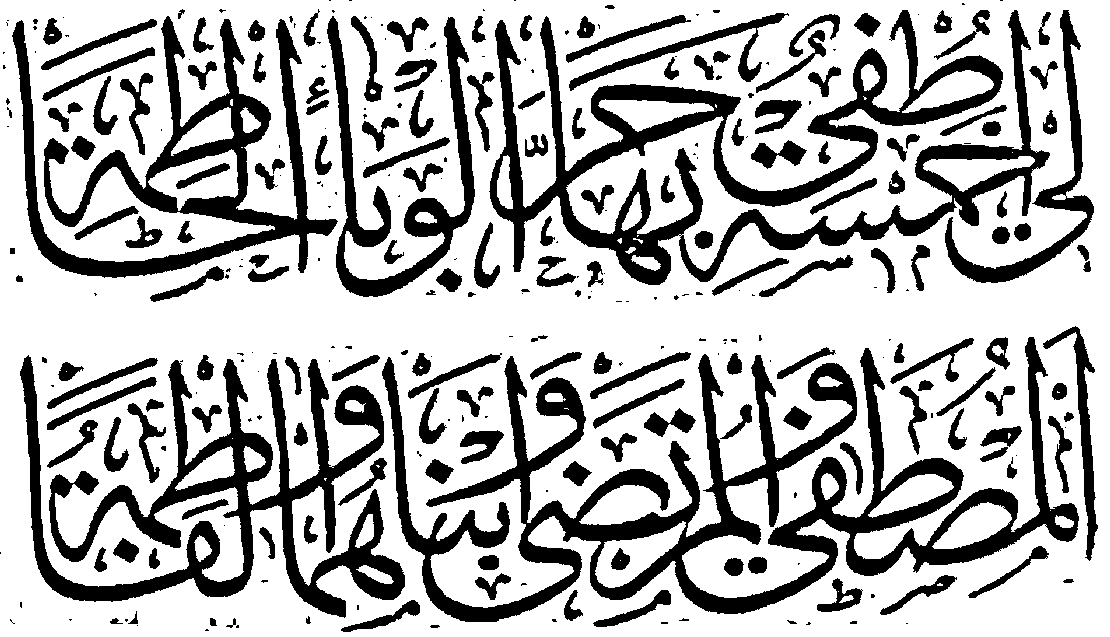
\includegraphics[width=0.25\textwidth]{images/nick_with_preprosseing.png} \\[0.4em]

\hline \\[-0.5em]

Sauvola &

\includegraphics[width=0.25\textwidth]{images/sauvola.png} &
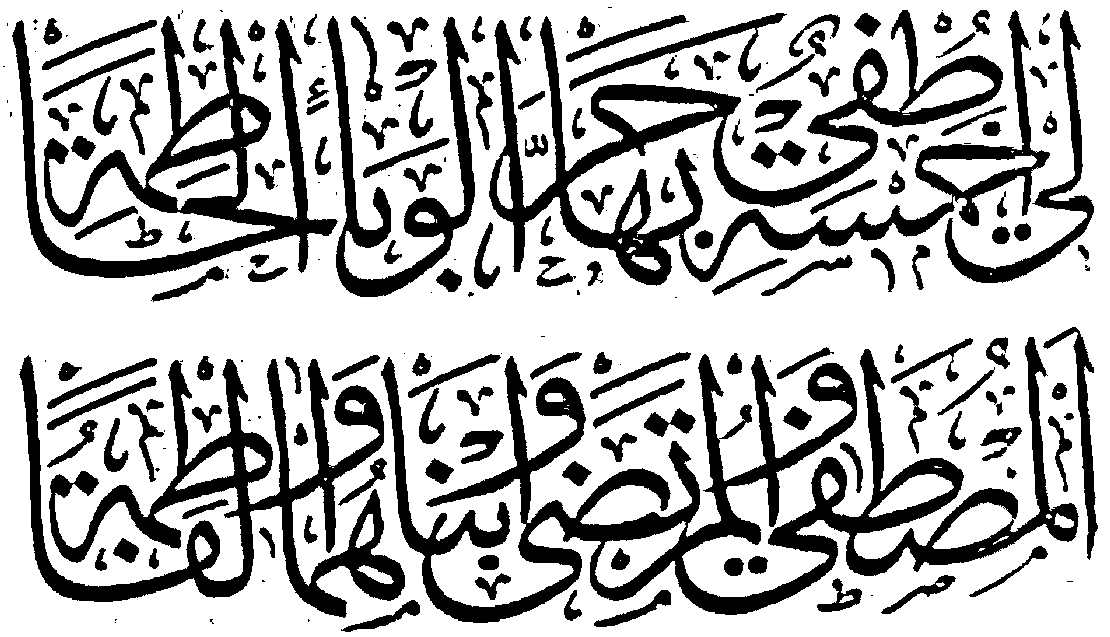
\includegraphics[width=0.25\textwidth]{images/sauvola_with_preprosseing.png} \\[0.4em]

\hline \\[-0.5em]

Su &

\includegraphics[width=0.25\textwidth]{images/su.png} &

\includegraphics[width=0.25\textwidth]{images/su_with_preprosseing.png} \\[0.4em]

\hline \\[-0.5em]

Proposed &

\includegraphics[width=0.25\textwidth]{images/proposed copy.png} &

\includegraphics[width=0.25\textwidth]{images/proposed_with_preprosseing.png} \\[0.4em]

\hline

\end{tabular}

\caption{Binarization results of all implemented methods, without and with preprocessing (contrast stretch percentile).}

\label{tab:binarization-results}

\end{figure}

\end{document}